\begin{frame}{self-supervised representation learning}{introduction}
    \begin{itemize}
        \item   \textbf{question}:
            \begin{itemize}
                \item   how can we provide extra training information without additional data labels (related approaches: transfer learning, multi-task learning)
            \end{itemize}
        \bigskip
        \item   \textbf{idea}: 
            \begin{itemize}
                \item use proven pre-trained features (e.g., VGGish, OpenL3)
            \end{itemize}
        \bigskip
        \item<2->   \textbf{goals}:
            \begin{itemize}
                \item   \textit{impart knowledge} of pre-trained deep models (VGGish, L3)
                \item   \textit{improve model generalization} by utilizing pre-trained features
                \item   use pre-trained features \textit{only during training}
            \end{itemize}
    \end{itemize}
\end{frame}

\begin{frame}{self-supervised representation learning}{method overview}
    \begin{figure}%
        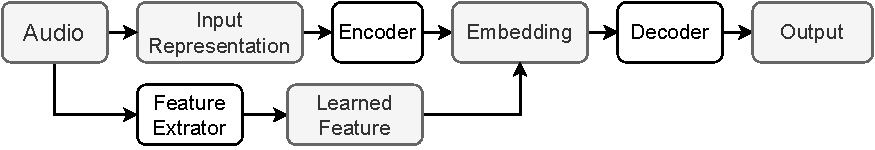
\includegraphics[width=.8\linewidth]{rep-pipeline}%
    \end{figure}
    \bigskip
    \begin{itemize}
        \item   \textbf{method 1: ``Con-Reg''}
            \begin{itemize}
                \item   make embedding space more similar to embedding space of features
            \end{itemize}
            \smallskip
        \item   \textbf{method 2: ``Dis-Reg''}
            \begin{itemize}
                \item   force distances between pairs of embedding vectors to be similar to feature distances 
            \end{itemize}
    \end{itemize}
\end{frame}

\begin{frame}{self-supervised representation learning}{experimental setup: baselines}
            \begin{itemize}
                \item   standard \textbf{transfer} learning
                    \begin{enumerate}
                        \item   extract features with pre-trained network
                        \item   train classifier for new task with feature input
                    \end{enumerate}
                    \bigskip
                \item   \textbf{concat}enation:
                    \begin{itemize}
                        \item   concatenate the pre-trained features and the learned embeddings
                        \item   classifier has the combined information (trained and pre-trained)
                    \end{itemize}
            \end{itemize}
\end{frame}

\begin{frame}{self-supervised representation learning}{experimental setup: data}
    \begin{columns}
        \column{.8\linewidth}
            \begin{itemize}
                \item   DCASE 17:
                    \begin{itemize}
                        \item   17 audio event classes
                        \item   \unit[10]{s} audio snippets ($\approx$ 53000)
                    \end{itemize}
                \bigskip
                \item   MagnaTagATune (MTAT):
                    \begin{itemize}
                        \item   50 music tags
                        \item   \unit[30]{s} audio snippets ($\approx$ 21000)
                    \end{itemize}
            \end{itemize}
        \column{.2\linewidth}
    \end{columns}
\end{frame}

\begin{frame}{self-supervised representation learning}{results: classification metrics}
    \vspace{-3mm}
    \begin{footnotesize}
    \begin{table}[]
        \centering
        \begin{tabular}{l l | c c c c | c c c c c}
           & Methods & \multicolumn{4}{c}{DCASE 17 (F1)} & \multicolumn{4}{c}{MTAT (PR-AUC)}\\
           \hline
           
           & & None & VGGish & OpenL3 & Combined & None & VGGish & OpenL3 & Combined \\
           \hline
           
           \multirow{4}{*}{BL} & Won et al.  &  0.547 & - & - & - & 0.465 & - & - & - \\
           
           & transfer & - & 0.496	& 0.477	& 0.501 & - & 0.454 & 0.454	& 0.456 \\
           
           & concat & - & 0.529 & 0.492 & 0.495 & - & 0.457 & 0.464 &	0.458\\
           
           %\midrule
           \hline
           
           \multirow{2}{*}{Prop.} & Con-Reg  & - & \underline{\textbf{0.568}} & \underline{\textbf{0.557}} & \underline{\textbf{0.576}} & - & \underline{\textbf{0.471}} & \underline{0.466} & \underline{\textbf{0.469}} \\
           
           & Dis-Reg & - & \underline{0.548} & 0.543 & \underline{0.563} & - & 0.464 & \underline{\textbf{0.468}} & 0.463 \\
          
        \end{tabular}
    \end{table}
    \end{footnotesize}
    
    \bigskip
    \begin{itemize}
        \item   two baselines \textit{cannot outperform} the trained system without additional features
        \smallskip
        \item   \textit{combining VGGish and L3 generally improves} on the individual feature results
        \smallskip
        \item   \textit{approach improves embedding space} by using pre-trained features during training
    \end{itemize}
    \phantom{\footfullcite{hung_feature-informed_2022}}
\end{frame}

\begin{frame}{self-supervised representation learning}{results: data dependency}
    \begin{itemize}
        \item   Con-Reg outperforms non-regularized system in all cases
        \item   larger improvement for lower amounts of data
    \end{itemize}
    \begin{figure}%
        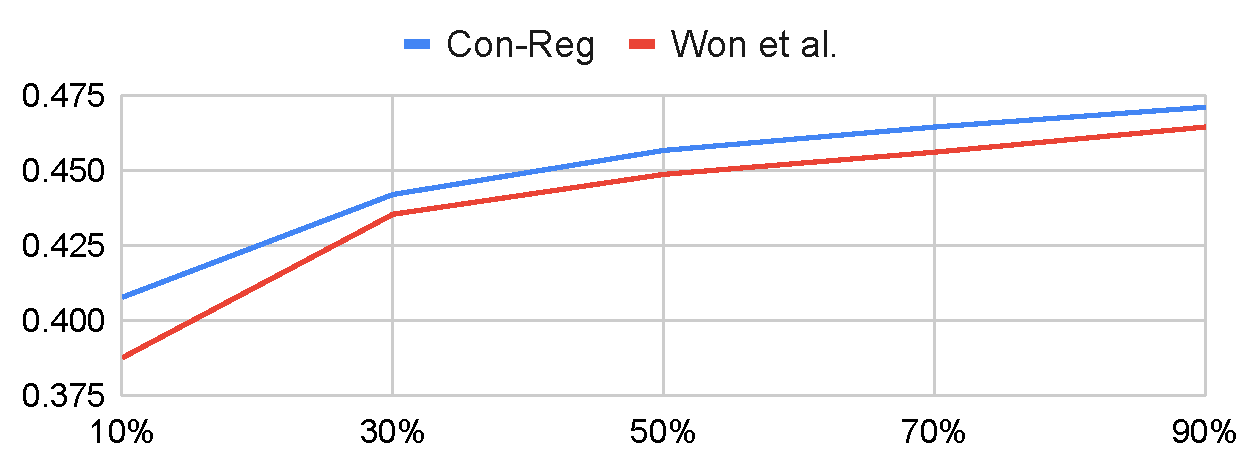
\includegraphics[scale=.45]{rep-results-data}
    \end{figure}
    
    \phantom{\footfullcite{hung_feature-informed_2022}}
\end{frame}
 